\documentclass[11pt,a4paper]{article}
\usepackage[margin=2.2cm]{geometry}
\usepackage[T1]{fontenc}
\usepackage{amsmath,amssymb,xcolor,enumitem,booktabs,graphicx,tabularx}
\usepackage[normalem]{ulem}
\setlength{\parskip}{0.6em}\setlength{\parindent}{0pt}
\definecolor{newc}{HTML}{1f6f43}
\newcommand{\new}[1]{\textcolor{newc}{#1}}
\newcommand{\old}[1]{\textcolor{gray}{\sout{#1}}}
\newcommand{\note}[1]{{\small\itshape [#1]}}
\newcommand{\lab}[1]{\textsf{\footnotesize\detokenize{#1}}}
\renewcommand{\ref}[1]{\lab{#1}}
\newcommand{\nref}[1]{\lab{#1}}
\newcommand{\citep}[1]{[\lab{#1}]}
\newcommand{\citet}[1]{\lab{#1}}
\newcommand{\mockup}[1]{\old{[#1]}}
\graphicspath{{review_results_red_text_files/}}
\title{Proposed text, the red text of the Experiments chapter and the appendix TODOs that can be written now}
\date{25 November 2026, version 3}
\begin{document}\sloppy
\maketitle

\section*{What changed in version 3}
\begin{itemize}[nosep]
  \item The multiple-tests paragraph is left out. The red text goes with no
    replacement.
  \item RQ3 becomes scale. The new wording of the research question, the
    factor, the expected outcome and the Experiments lines is in section 6.
    It changes a research question, so it gets a GAPS entry when applied
    ([A139]).
  \item 8 agents at 18\,\%. Two sentences change wording, since the gain now
    shows on every seed (section 2).
  \item NordLocker is not named.
\end{itemize}

\section*{What changed in version 2}
\begin{itemize}[nosep]
  \item Your answers are in. Holm is not named. The untested reward sweeps
    of Appendix~I go (the fleet reward test is separate and stays). Size and
    dock ratio are argued, not run. Appendix~K states the checks in words.
    Appendix~G keeps its first test. The backlog trace and the crowding
    scatter are dropped. The served share is recounted.
  \item New. The 16-agent policies played at 8, 32 and 64 agents are named
    as the scalability test, a policy learned in a small warehouse played in
    a larger one (Setup, RQ3, Discussion).
  \item New. Token Passing on the test seeds at every fleet. At 8 agents this
    changes the gain from 14.1\,\% to 18.4\,\% (section 2). 32 and 64 agents
    are queued on the Lenovo after the lock replay.
  \item Applied already. The $|V|$ column of \lab{tab:app:window} (368, 736,
    1472).
\end{itemize}

\section*{How to read this}
Every red \texttt{\textbackslash mockup} of \lab{5.Experiments.tex} and every
appendix TBD or TODO was checked against the data on disk. This review holds
the ones that can be written now, from finished runs or as text only. Black
text stays, \new{green} is new and \old{struck} text goes (a struck
\old{[...]} is the red mock-up it replaces). \note{Notes in brackets} say where
a number comes from. Nothing below is in the thesis yet.

Not here, because they wait for runs: ``Fixed and demand storage'' under RQ1,
the controller, and the [A110], [A112] and [A123] TODOs (centralised demand
still evaluating on eval-pc), Appendix~L at 16 agents rebuilt on the long
runs, the stall recount of Appendix~H, and every lock count (Lenovo replay,
[A136]). The questions are at the end.

\begin{enumerate}[nosep]
  \item Setup. The load row, seeds, tuning, warm-up, pairs, run plan, compute.
  \item Results. 32 and 64 agents, training curves, RQ3, training time.
  \item Discussion. RQ3, earlier work, threats to validity.
  \item Appendices E, H, I and L.
  \item One finding to check first. The served share at 32 and 64 agents.
\end{enumerate}

% ==================================================================
\section*{1. Motivation and Setup (\lab{sec:exp:setup})}

\textbf{Table \lab{tab:expfactors}, the load row.}

\begin{tabular}{lll}
  \toprule
  Factor & Values & Research question \\
  \midrule
  load & \old{$m \in$ [TBD], $\lambda_{\mathrm{task}} \in$ [TBD]}
         \new{$m \in \{8, 16, 32, 64\}$, each at its main load} & RQ3 \\
  \bottomrule
\end{tabular}

\note{Appendix E sets one main load per fleet, 0.6 of Token Passing's capacity,
0.09, 0.18, 0.3 and 0.6 tasks per step. The arrival rate was swept only for
Token Passing under fixed storage, so it is not a factor of the main design.}

\textbf{Mapping questions to comparisons.} \old{[Table mapping each RQ to the
runs compared and the measure read, if the paragraph is not enough.]}
\note{Dropped. The paragraph already names the pair and the measure of each
question.}

\textbf{Training.} \old{[Number of training seeds per controller and storage
rule. Whether one policy is trained for each load level and congestion
setting, or one policy is trained once and evaluated at every load.]}
\new{Each controller and storage rule has one training run, so twelve
policies are trained, all at 16 agents and at its main load. Training a set
of policies for every fleet size did not fit the time and compute
available. The policies trained at 16 agents therefore also play the 8, 32
and 64-agent warehouses, on their own test seeds and main loads. This is the
test of scale. A graph network reads a warehouse of any size, so one policy
can play every fleet. A policy that learned how to move a fleet, and not
just one warehouse size, should then keep up in the larger warehouses too.
The seed counts, steps and episode lengths are in
Table~\ref{tab:trainparams}.}
\note{Your note of today. No new training table, Appendix B already has the
numbers. Decision time at 128 agents uses the same policies.}

\old{[How the values left open in Tables storageparams, rlparams and
trainparams are tuned, on which seeds and with what budget per controller, so
that tuning does not favour one controller.]}
\new{No value is tuned for one controller. Every value in these tables was
set once, before any learned controller was trained, and every controller
trains with the same values. The storage values come from sweeps of Token
Passing, the learning values from cited sources, and the reward weights are
set without a test (Appendix~\ref{app:parameters}).}

\textbf{Scoring a condition.}
\old{[Warm-up. A run starts with no tasks, and the storage rule needs data
before its first useful update, so the first timesteps are not typical. State
how many are discarded before scoring, and that $T$ covers many storage
periods.]}
\new{A run starts with no tasks and the storage rule has no demand to read
yet, so its first steps are not typical. The first 5000 of the 10000 steps
are therefore left out. The 5000 steps that are scored hold 50 storage
updates and 25 shifts of demand (Appendix~\ref{app:horizon}).}

\old{[What a pair is when the two runs use different policies, as under
matched training. Either pair by training seed and evaluation seed, or average
over training seeds first.]}
\new{Under each rule the controller plays the policy trained under that rule.
A pair is then the same test seed played by two policies. There is one
training run per policy, so nothing is averaged over training runs first.}

\old{[How many gain tests are run in total, and whether a correction for
multiple comparisons, such as Holm's, is applied.]}
\note{Left out, no replacement (your answer).}

\textbf{Run plan.} \old{[Number of trained policies and of evaluation runs
\ldots\ the number of evaluation seeds, from the variance of the gain they
show.]}
\new{Twelve policies are trained at 16 agents, four controllers under three
rules, each in the two stages above. Every third checkpoint plays the 5
validation seeds, and the chosen one plays the 20 test seeds. Token Passing
plays the same 20 test seeds under each rule. The load of each fleet comes
from a load sweep of Token Passing under fixed storage, from light load to
past the rate it can serve (Appendix~\ref{app:load}). Twenty seeds give an
interval on Token Passing's gain of 3 to 6 points either side, far narrower
than the gain.}
\note{The number 20 was not chosen from a variance pilot. The last sentence
gives the reason it suffices, after the fact. Remove it if that reads as a
claim.}

\textbf{Compute environment.}
\old{[Where the code version, configuration files, trained checkpoints and
raw per-run results are archived.]}
\new{The code and the configuration files are in the repository
\texttt{slap-mapd-coupling}, and the scripts that make every table and figure
in \texttt{thesis-progress}. The trained checkpoints and the per-run results
are kept with the runs, and the files too large for the repositories are
archived apart.}

Table \lab{tab:exp:compute}. Training ran on four machines, so I propose one
column per machine.

\begin{tabularx}{\linewidth}{l>{\raggedright\arraybackslash}X>{\raggedright\arraybackslash}X>{\raggedright\arraybackslash}X}
  \toprule
  & PC & Lenovo & Kaggle, Colab \\
  \midrule
  \new{use} & \new{training, evaluation, decision time} & \new{evaluation} & \new{training} \\
  \new{CPU} & \new{Intel i7-9700K, 8 cores} & \new{Intel i5-9500T, 6 cores} & \new{as provided} \\
  \new{memory} & \new{32 GB} & \new{12 GB} & \new{as provided} \\
  \new{GPU} & \new{NVIDIA RTX 2070 Super, 8 GB} & \new{none} & \new{[Kaggle GPU], NVIDIA L4 24 GB} \\
  \new{system} & \new{Linux 7.2 (Garuda)} & \new{Debian 13} & \new{as provided} \\
  \bottomrule
\end{tabularx}

\new{software} Python 3.10, PyTorch 2.13 (CUDA 12.6), Ray RLlib 2.57.
\new{code version} training on commit 6dbe094 (and 8478c99 for the cloud
parts), evaluation on 131b6b1. \new{parallelism} 3 rollout workers, one
environment each. \new{training time} see section 2, Costs.
\new{runtime measurement} the PC, learned controllers on its GPU, Token
Passing on one CPU thread.
\note{Kaggle GPU model to fill in. Commits from each run's \texttt{done} and
\texttt{commit.txt}. Check the evaluation commit wording, since 131b6b1 is not
on main.}

% ==================================================================
\section*{2. Results (\lab{sec:exp:results})}

\textbf{Opening.} \ldots are in Appendix~\ref{app:results:tests}.
\old{[32 agents, in the same appendix once tested.]}
\new{Played in the larger warehouses, the policies trained at 16 agents fall
behind on every seed at 32 and 64 agents, while Token Passing keeps up.}
\note{Recounted served share, section 5. Token Passing's 32 and 64-agent gains
follow once the test-seed runs are in.}

\textbf{Opening, first sentence.} Demand storage makes Token Passing's orders
\old{14\,\%} \new{18\,\%} faster at 8 agents and 20\,\% faster at 16.
\note{Test seeds at every fleet (your answer to question 7). The same change in
RQ1, storage adaptation (``The gain is \old{14\,\%} \new{18\,\%} at 8 agents'')
and the first sentence of the Discussion (``\old{14 to 20\,\%}
\new{18 to 20\,\%} faster''). The Abstract and Conclusion have no number.
Nothing in the argument changes. The gain is a little larger, and 8 and 16
agents are now closer.}

\textbf{RQ1, storage adaptation.} The gain is \old{14\,\%} \new{18\,\%} at 8
agents and 20\,\% at 16, and it shows on \old{nearly} every seed.
\note{Test seeds, 20 of 20 at both fleets. The congestion-aware column is 19
of 20 at 8 agents.}

\textbf{Training.} \old{[Learning curves of the three learned controllers
under each storage rule. State whether all three reached a stable return
within the budget, and whether training under demand and congestion-aware
storage was harder, as Section training expects.]}
\new{Figure~\ref{fig:exp:learning} shows how many tasks each policy finished
per step during the long training stage. The training return is not shown,
because the shaping term dominates it. Under congestion-aware storage every
controller climbs to about 0.22 to 0.25 tasks per step, close to Token
Passing's 0.29. Under fixed and demand storage the curves spread out, and the
decentralised controller stays below 0.1 for the whole run. Several runs are
still rising at 2 million steps, among them the centralised controller under
fixed and demand storage. So not every run has settled within the budget.}

\begin{center}
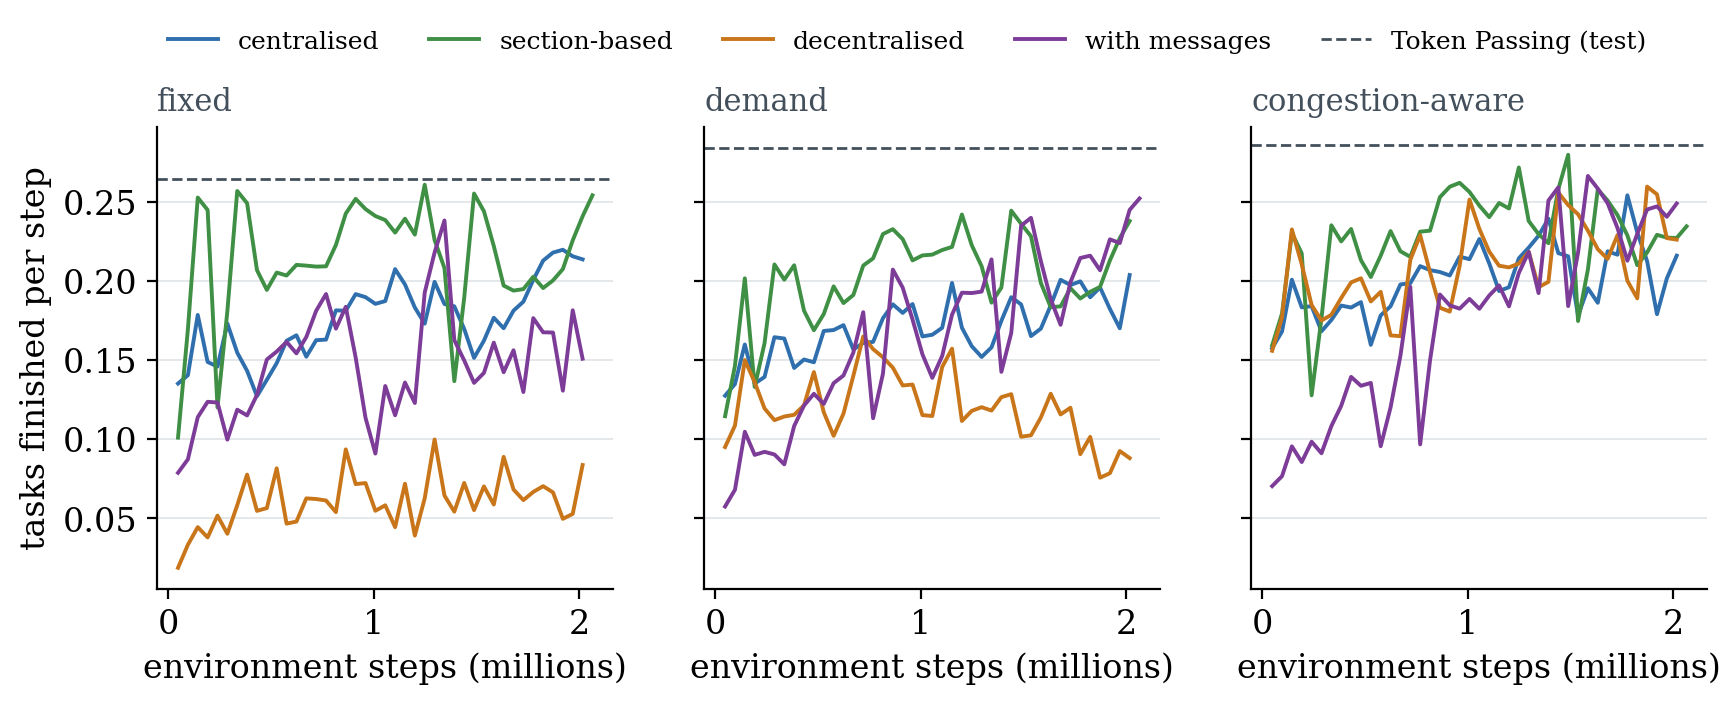
\includegraphics[width=\linewidth]{learning.png}
\end{center}
\new{Caption. Tasks finished per step in the long training of each learned
controller at 16 agents. The dashed line is Token Passing in the test runs.}
\note{Draft, to redraw in thesis-progress. Training episodes are 16\,000 steps,
the test 10\,000, so the dashed line is a guide, not a pair. The figure
replaces the mock-up of mean return.}

\textbf{Dropped figures.} \old{[Backlog trace of one condition that falls
behind.]} (Keeping up) and the figure \old{[Crowding against mean service
time]} (RQ2) go. Figure \lab{fig:exp:split} becomes panel (b) of the RQ3
figure, Token Passing only, since the learned runs fall behind and their wait
is mostly queue.

\textbf{RQ3, scale.} \old{[Gain against fleet size and arrival rate. Mark the
load at which each controller and storage rule stops keeping up.]}
\new{Demand storage keeps its gain for Token Passing as the fleet grows. At
each fleet's main load an order gains 18\,\% at 8 agents, 20\,\% at 16,
[TBD] at 32 and [TBD] at 64 (Figure~\ref{fig:exp:rq4}). The time saved is
travel and the wait for an agent at every size. Blocked time stays near 2
steps per pick.}

\new{The learned policies do not carry over to larger warehouses. Trained at
16 agents, they keep up at 8 agents on 15 to 18 of the 20 seeds. At 32
agents they serve 0.28 to 0.63 of the work and at 64 agents 0.28 to 0.45,
and none keeps up on any seed. So what they learned at 16 agents does not
scale, and their gain can be measured at no fleet size.}
\note{Learned, congestion-aware policies of the perf test, recounted. Token
Passing 32 and 64 follow the Lenovo runs. Heading ``load'' becomes ``scale'',
section 6.}

\begin{center}
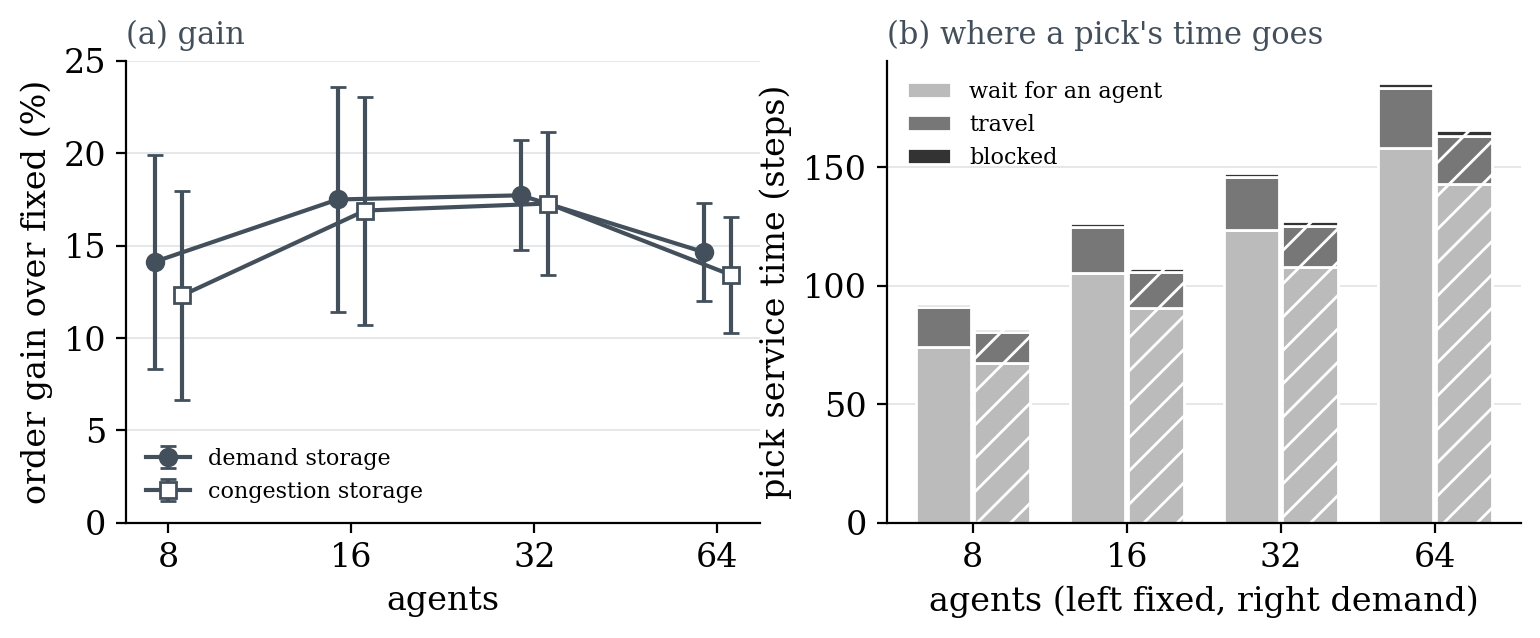
\includegraphics[width=\linewidth]{tp_fleet.png}
\end{center}
\new{Caption. Token Passing at each fleet's main load. (a) The order gain of
demand and congestion-aware storage, with 95\,\% intervals. (b) Where a
pick's time goes.}
\note{Draft on seeds 0 to 19. Redrawn on the test seeds once 32 and 64 are in.}

Table \lab{tab:exp:rq1}, all on the test seeds. \note{The 8 row changes, 16
stays, 32 and 64 follow the Lenovo runs. Seeds 0 to 19 gave 17.7\,\% at 32
and 14.6\,\% at 64, so expect similar values.}

\begin{tabular}{l c cc cc}
  \toprule
  fleet & $\bar\zeta_T$ under $F_{\mathrm{fix}}$ & gain of $F_{\mathrm{dem}}$ & seeds faster
    & gain of $F_{\mathrm{cng}}$ & seeds faster \\
  \midrule
  8 agents  & \old{177.5} \new{216.1} & \old{14.1\,\% [8.3, 19.9]} \new{18.4\,\% [13.1, 23.7]} & \old{18} \new{20} & \old{12.3\,\% [6.7, 18.0]} \new{16.5\,\% [11.8, 21.1]} & \old{17} \new{19} \\
  16 agents & 278.9 & 20.0\,\% [16.0, 24.1] & 20 & 19.9\,\% [15.0, 24.9] & 20 \\
  32 agents & \new{[Lenovo]} & \new{[Lenovo]} & & \new{[Lenovo]} & \\
  64 agents & \new{[Lenovo]} & \new{[Lenovo]} & & \new{[Lenovo]} & \\
  \bottomrule
\end{tabular}

\textbf{Costs.} \ldots\ to reach the best shelves.
\old{[Training time per controller, as in Section impl:cost.]}
\new{Training time follows the same order as decision time. On the PC the
first stage of 500\,000 steps took about 8 hours for the centralised
controller, 6 for the section-based, 3 with messages and 2 to 3 without. The
long stage of 2 million steps took 25 to 41 hours per run, on several
machines, so these times are not compared. All training took about 500
hours.}
\note{Sum of \texttt{time\_this\_iter\_s} per run. 500 h includes aborted
cloud starts.}

% ==================================================================
\section*{3. Discussion (\lab{sec:exp:discussion})}

\textbf{What was expected.} \ldots\ Messages helped only under fixed storage.
\old{[RQ3, once the larger fleets are tested.]}
\new{The gain of demand storage held as the fleet grew, as expected, for
Token Passing from 8 to 64 agents. The learned policies were trained only at
16 agents, because training at every size did not fit the time and compute
available. Played in larger warehouses they fall behind, so the test of scale
shows that what they learned is tied to the size they trained at.}

\new{A policy that carries over would make training at scale unnecessary,
and that is what the test asks. The decentralised controller reads a window
of the same size at every fleet, so it might be expected to carry over best.
It does not. At 32 agents it serves less than the centralised controller.}
\note{Check against the lock discussion once the fleet reward review lands.}

\textbf{Relation to earlier work.} \ldots\ where the learned controllers fall
behind.
\old{[Compare with lifelong MAPD, the GCN routing of van Knippenberg and
crowd-aware routing.]}
\new{Token Passing comes from the lifelong MAPD work of
\citet{ma2017lifelong_mapf}, who show that it never deadlocks in a
well-formed warehouse. Every warehouse here is well-formed, so it never
locking is what they predict. \citet{vanKnippenberg2021} route with a GCN up
to 128 agents, but their agents share part of the reward and pay more for
waiting than for moving. Here waiting is the cheaper choice, which helps
explain the locks. \citet{pham2024optimizingcrowdawaremultiagentpath} also
train decentralised agents that pass messages through a graph network. They
add a reward for the whole team, a penalty for hindering others and a
reward for avoiding crowds, and their success falls sharply at 32 and 64
agents once the crowd-aware reward is removed. Their agents trained up to 8
agents only, as ours trained at 16.}
\note{From the lock discussion of 2026-11-25. Check it does not repeat the
Discussion paragraph on why the learned controllers fall behind once the
fleet reward text lands.}

\textbf{Threats to validity.} \old{[Each in a sentence or two.]}
\begin{itemize}
  \item \old{[Stored stock never moves, so cold stock can hold the best shelves.]}
    \new{Stored stock never moves (Section~\ref{sec:pf:scope}). A SKU that
    turns cold keeps its shelf near the workstations until it is picked
    empty, so demand storage gains less than a rule that also moves stock
    would.}
  \item \old{[Congestion-aware storage changes where new stock goes and which
    shelf a pick uses at once, so RQ2 cannot say which of the two helped.]}
    \new{Congestion-aware storage changes two things at once, where new stock
    goes and which shelf a pick takes. RQ2 cannot say which of the two
    helped.}
  \item \old{[All instances come from one generator \ldots]}
    \new{Every warehouse comes from one generator. The results hold for that
    family of layouts, not for warehouses of another shape.}
  \item \old{[The policy cannot tell neighbours apart by vertex number, only
    by their features.]}
    \new{An agent knows its neighbours only by their features, not by which
    vertex they are (Section~\ref{sec:method:model}). Two places that look
    the same are treated the same, which lets one policy play every
    warehouse but hides where in the warehouse an agent stands.}
  \item \old{[A finite training budget \ldots]}
    \new{Several runs were still improving when training stopped
    (Figure~\ref{fig:exp:learning}). A longer budget could narrow the gap to
    Token Passing.} \note{Merged with the budget remark, so the threat says
    it once.}
  \item \old{[Values left open in Chapter method and fixed by a sweep may
    favour one controller.]}
    \new{The storage values were set by sweeps of Token Passing. They may
    suit a planner better than a learned controller. The delivery reward,
    the override penalty and the crowding weight were set without a test.}
  \item \new{Every warehouse gives each agent 16 walkable vertices and each
    dock two agents. Neither ratio is varied, so whether the result depends
    on them is open.}
  \item \new{The policies were trained at 16 agents only. A policy trained at
    32 or 64 agents might keep up there, so the test of scale says how far a
    policy carries over, not how well a controller can do at that size.}
\end{itemize}

% ==================================================================
\section*{4. Appendices}

\subsection*{Appendix L, 8 agents} \note{See question 5 before this goes in.}
\note{The rows exist under \texttt{\textasciitilde/thesis\_runs/evaluation/fleet\_8}.
\texttt{appendix\_results.py} reads them from another folder, so every table
stayed TBD. Built with \texttt{served\_counts.py} at $f_{\mathrm{up}} = 0.9$.
The keep-up counts match the [A111] TODO exactly. The stalled column is
counted here as a stretch of more than 400 steps with no task finished,
because the runs left it unset. Every other table (service time, cost,
backlog, stock) is filled the same way, in
\texttt{review\_results\_red\_text\_files/tables8.tex}.}

Table \lab{tab:app:check}, all rows new.

{\small\setlength{\tabcolsep}{4pt}
\begin{tabular}{llrrrrr}
  \toprule
  rule & controller & picks keep up & put-aways keep up & served & backlog slope & stalled \\
  \midrule
  fixed      & Token Passing & 20 of 20 & 20 of 20 & 0.98 & $-0.03$ & 0 \\
             & centralised   & 7 of 20  & 6 of 20  & 0.86 & 2.27 & 0 \\
             & section-based & 11 of 20 & 11 of 20 & 0.87 & 1.99 & 0 \\
             & decentralised & 11 of 20 & 9 of 20  & 0.84 & 2.43 & 2 \\
             & with messages & 15 of 20 & 15 of 20 & 0.96 & 0.62 & 0 \\
  demand     & Token Passing & 20 of 20 & 20 of 20 & 0.99 & $-0.01$ & 0 \\
             & centralised   & 10 of 20 & 8 of 20  & 0.90 & 1.80 & 0 \\
             & section-based & 9 of 20  & 8 of 20  & 0.81 & 2.94 & 1 \\
             & decentralised & 11 of 20 & 9 of 20  & 0.87 & 2.04 & 0 \\
             & with messages & 5 of 20  & 5 of 20  & 0.66 & 4.57 & 3 \\
  congestion & Token Passing & 20 of 20 & 20 of 20 & 0.99 & $-0.00$ & 0 \\
             & centralised   & 6 of 20  & 5 of 20  & 0.81 & 2.96 & 0 \\
             & section-based & 11 of 20 & 11 of 20 & 0.91 & 1.58 & 0 \\
             & decentralised & 11 of 20 & 11 of 20 & 0.82 & 2.49 & 3 \\
             & with messages & 11 of 20 & 10 of 20 & 0.82 & 2.64 & 2 \\
  \bottomrule
\end{tabular}}

\new{At 8 agents no learned controller keeps up on every seed. They serve
0.66 to 0.96 of the work. The controller with messages under fixed storage
comes closest, keeping up on 15 of the 20 seeds. A run that stalls belongs to
a decentralised controller, with or without messages, in all but one case.}
\note{Replaces nothing, a new paragraph after the opening one of the 8-agent
subsection. The [A111] TODO goes.}

\subsection*{Appendix E, the lower rates}
\new{Every rate below a fleet's capacity was played again with the served
counts and keeps up on all 20 seeds at $f_{\mathrm{up}} = 0.9$.}
\note{\texttt{results/E\_load/fleet\_<m>/served\_check\_low}. 0.1 and 0.125
at 8, 0.2 and 0.25 at 16, 0.4 at 32, 0.8 at 64. The TODO goes.}

\subsection*{Appendix H, the answer and the two figures}
Summary, in place of the TODO:
\new{Over a short run the gain is not yet settled. At 16 agents it ranges
from a loss of 0.2 to a gain of 0.3 within 20 drift periods, so a run must
hold many shifts of demand. With 25 drift periods after a warm-up of 5000
steps every reported run is past that point.}

After the figures, in place of the TODO:
\new{The backlog jumps at each shift of demand and falls again before the
next (Figure~\ref{fig:app:horizontrace}). At 8 and 16 agents it stays level,
and at 32 and 64 agents it still creeps up over the first 4000 steps, which
is why the warm-up is long. The gain moves most at short horizons and steadies
from about 15 drift periods (Figure~\ref{fig:app:horizongain}).}
\note{Both figures are from the earlier graph of 24 October, as their captions
say.}

\subsection*{Appendix I, the window and the discount}
Table \lab{tab:app:window}, new cells.

\begin{tabular}{rrrr}
  \toprule
  $m$ & $|V|$ & vertices in the field of view & share of $V$ \\
  \midrule
  8  & 184               & \new{25.9} & \new{14.1\,\%} \\
  16 & \old{348} \new{368}  & \new{27.5} & \new{7.5\,\%} \\
  32 & \old{676} \new{736}  & \new{27.3} & \new{3.7\,\%} \\
  64 & \old{1352} \new{1472} & \new{28.6} & \new{1.9\,\%} \\
  \bottomrule
\end{tabular}

\note{Current generator, test seeds 200000 to 200004, mean over every vertex
an agent can stand on, not over agents and steps. The caption should say that.
The $|V|$ column does not match what the generator builds now. Check against
\lab{tab:instances} before applying. Question 8.}

\new{An agent sees about 27 vertices at every fleet size, because the
warehouse grows by adding blocks of the same depth. That is a seventh of the
warehouse at 8 agents and a fiftieth at 64.} \note{In place of the depth TODO.}

\textbf{Discount.} The text already gives the source and the reason. The two
TODOs go.

\textbf{The reward sweeps go.} They never ran. The fleet reward test is a
different test and is not touched here.
\begin{itemize}[nosep]
  \item Summary. The delivery reward, the override penalty and the crowding
    weight have no source and \old{are set by training runs on the 8-agent
    warehouse} \new{are not tested}.
  \item Method. Here the delivery reward is paid for every completed task,
    \old{so a pilot compares $n_{\mathrm{deliver}}$ of 1 and 10} \new{so its
    size is a choice. It is set to 10, the value of their episode reward}.
  \item Method. The whole paragraph \old{For the crowding weight, a short
    training run first logs the mean of each reward term per step \ldots\ the
    smallest that lowers blocked time without lowering throughput.} goes.
  \item Results. \old{Calibration: the reward weights}, its TODO, the two
    figures \lab{app_reward_terms.png} and \lab{app_reward_cng.png} and
    \lab{tab:app:deliver} go.
  \item Conclusion. \new{The step costs are cited and are not tested. The
    observation depth of 5 comes from \citet{vanKnippenberg2021}, and an
    agent sees about 27 vertices at every fleet size. The discount of 0.99
    comes from \citet{schulman2017ppo}. The delivery reward, the override
    penalty and the crowding weight are set without a test, and every
    controller trains with the same values.} \old{The delivery reward, the
    override penalty and the crowding weight stay open until their training
    runs are done.}
\end{itemize}
\note{Appendix B, Source column. $n_{\mathrm{deliver}}$, $n_{\mathrm{override}}$
and $n_{\mathrm{crowd}}$ become ``set, not tested''. Check the Method chapter
does not promise the sweep.}

\subsection*{Appendix D, size and dock ratio}
In place of the two TODOs, after ``Whether the main result depends on that
ratio is open.'':
\new{Neither ratio was varied. The size of 16 walkable vertices per agent
follows \citet{vanKnippenberg2021} and keeps the space per agent the same at
every fleet. Two agents per dock spread the arrivals, and Token Passing
finishes its put-aways on every seed at every fleet, so the docks do not
limit it at the main load.}

\subsection*{Appendix K, the checks}
\lab{tab:app:checks} and its TODO go. In their place:
\new{Every reported run finished. The first two checks run at every step and
stop a run that fails, so no reported run broke them. A task's stage is read
from its times, so the third check holds by how the simulator is built.
Test seeds that were played again gave the same rows as their first runs.}
\note{The last sentence. The lock replays check every row against its first
run, so I confirm it when \texttt{collect.py} runs.} The timing figure
\lab{app_timing.png} and its TODO go, pointing instead to the step time of
Appendix~\ref{app:results:scaling}.

\subsection*{Appendix G, the congestion test}
The first test stays as written. Only the TODO goes.

% ==================================================================
\section*{5. The served share at 32 and 64 agents (agreed)}

The perf test rows (\texttt{results/L\_results/scaling/perf/rows}) were written
on main bdfda94, which does not yet count the order lines still waiting for
stock at the end. SESSION\_CONTEXT's numbers come straight from the rows'
\texttt{served\_share}. At 32 and 64 agents many lines wait for stock. One
64-agent row has 2798 such lines and a pick share of 3.4, which is impossible.
Recounted with \texttt{served\_counts.py}, as every other run is:

\begin{tabular}{lcccc cccc}
  \toprule
  & \multicolumn{4}{c}{rows as written} & \multicolumn{4}{c}{recounted, [A96]} \\
  \cmidrule(lr){2-5}\cmidrule(lr){6-9}
  controller & 8 & 32 & 64 & & 8 & 32 & 64 & \\
  \midrule
  centralised    & 1.00 (18) & 0.84 (2) & 0.94 (18) && 0.99 (17) & 0.63 (0) & 0.45 (0) \\
  section-based  & 0.99 (18) & 0.87 (7) & 0.94 (17) && 0.98 (16) & 0.51 (0) & 0.35 (0) \\
  decentralised  & 0.97 (17) & 0.79 (2) & 0.70 (3)  && 0.96 (15) & 0.53 (0) & 0.32 (0) \\
  with messages  & 0.99 (19) & 0.51 (1) & 0.69 (10) && 0.99 (18) & 0.28 (0) & 0.28 (0) \\
  \bottomrule
\end{tabular}

Served share, seeds that keep up in brackets. Recounted, the odd ``32 worse
than 64'' goes away. Every learned controller serves less as the fleet grows,
and none keeps up at 32 or 64. The text above uses the recounted numbers.
These are the policies trained at 16 agents, played in the larger warehouses
(the test of scale). 128 agents is played for decision time only.

% ==================================================================
% ==================================================================
\section*{6. RQ3 becomes scale}
The arrival rate is never varied, and the larger fleets play the policies
trained at 16 robots. So RQ3 asks about scale. Each change below, in the
order a reader meets it.

\textbf{Introduction, the factors.}
\old{the load: the number of robots and how fast orders arrive, as a share of
what the fleet can serve}
\new{the scale: the number of robots, with the warehouse growing in step,
each at a load the fleet can serve}

\textbf{Introduction, RQ3.}
\old{As orders arrive faster, does the gain of RQ1 grow, shrink or disappear,
and at what rate does each learned controller stop keeping up?}
\new{As the warehouse and its fleet grow, does the gain of RQ1 hold, and does
a controller trained on 16 robots still keep up in a larger warehouse?}

\textbf{Introduction, expected outcome.}
\old{For RQ3, the gain should hold as orders arrive faster and stop near the
rate where the fleet no longer keeps up.}
\new{For RQ3, the gain should hold as the warehouse grows, because every
size gives each robot the same space and aisles of the same depth.}
The decentralised controller should stop keeping up first, because each
robot decides alone and runs into more conflicts.
\note{The second sentence is kept as it stands, so the prediction made before
the runs does not change. The results then say whether it held. At 32
agents the controller with messages serves least, and without messages it
serves about as much as the section-based one.}

\textbf{Experiments, the gain test.} How the gain holds as
\old{the load grows} \new{the warehouse grows} is RQ3.

\textbf{Experiments, mapping questions to comparisons.}
\old{RQ3 repeats the comparison across load levels and records the load at
which each pair stops keeping up.}
\new{RQ3 repeats the comparison at 8, 32 and 64 agents, with the policies
trained at 16, and records whether each still keeps up.}
On the same runs it reads throughput per agent, $\Lambda_T / m$.

\textbf{Experiments, \lab{tab:expfactors}.}

\begin{tabular}{lll}
  \toprule
  \old{load} \new{scale} & $m \in \{8, 16, 32, 64\}$, each at its main load & RQ3 \\
  load for the loop & main load, 0.9 of capacity & RQ2 \\
  \bottomrule
\end{tabular}

\textbf{Experiments, results.} The heading \old{RQ3, load} \new{RQ3, scale}.
\note{GAPS [A139]: RQ3 asks about scale, because the arrival rate was never
varied and training at every size did not fit the time and compute. RQ2 keeps
its higher load.}

\section*{Questions}
\begin{enumerate}
  \item \textbf{8-agent tables of Appendix L.} On 23 November you decided that
    8 agents appears only through the scale test with the 16-agent policies.
    The keep-up table of section 4 comes from the earlier runs trained at 8
    agents, which goes against that. Either fill the 8-agent tables from the
    scale test (congestion-aware policies only, so the fixed and demand rows
    stay empty), or keep the earlier runs there as now. Recommended the
    scale test, which also matches the Results text.
  \item \textbf{Apply?} If versions 2 and 3 read right, I apply everything
    except what waits for runs (the Lenovo, centralised demand, the lock
    count), with the GAPS entry.
\end{enumerate}

\end{document}
